	% Use standalone to generate PDF images
	% Recommended in slower machines and big files!
\documentclass{standalone}

	% Standard LaTeX libs
	%\usepackage{amssymb}

	% Custom TikZ
\usepackage{tikz}
\usetikzlibrary{3d}

	% Enable if using Overleaf to speed up compialtion times
	%\usepgfplotslibrary{external}
	%\tikzexternalize

\begin{document}
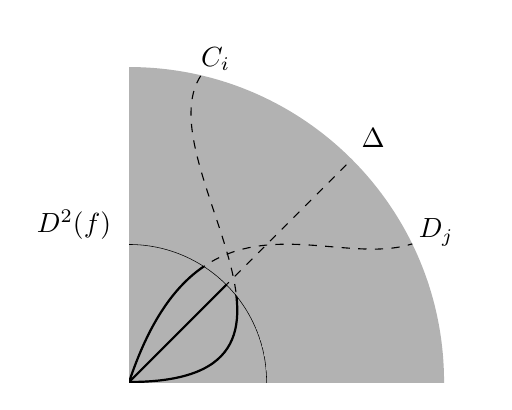
\begin{tikzpicture}
	\draw (-.7,2) node {$D^2(f)$};

	% The circle that stands for D^2(f)
	\clip (0,0) rectangle (4.5,4.5);
	\draw[fill=black!30,draw opacity=0] (0,0) circle (4cm);

	% The ball where the curves only meet at the origin
	\begin{scope}
	\clip (0,0) circle (4cm);
	\draw[dashed] (0,0) -- (4,4);									%Delta
	\draw[dashed] (0,0) .. controls (3,0) and (0,3) .. (1,4);		%C
	\draw[dashed] (0,0) .. controls (1,3) and (3,1) .. (4,2);		%D
	\end{scope}

	% The outside of the ball	
	\begin{scope}
	\clip (0,0) circle (1.75cm);
	\draw (0,0) circle (1.75cm);
	\draw[thick] (0,0) -- (4,4);									%Delta
	\draw[thick] (0,0) .. controls (3,0) and (0,3) .. (1,4);		%C
	\draw[thick] (0,0) .. controls (1,3) and (3,1) .. (4,2);		%D
	\end{scope}

	\draw (3.1,3.1) node {$\Delta$};
	\draw (1.1,4.1) node {$C_i$};
	\draw (3.9,1.9) node {$D_j$};
\end{tikzpicture}
\end{document}
